\subsection{Product perspective}

\textit{Travlendar+} is a mobile application that’s going to be built from scratch and heavily reliant on external APIs. 
We’ll start with open, official immediately accessible APIs : one that contitues the core of Travel Logic, and one as a reference for the implementation of car-sharing rental. 
Tavlendar+ has to implement a modular approach, so that later on it will be able to implement and expand upon iterative additions of external services as its operative zone grows and new partnerships arise.
In its firts version, \textit{Travlendar+} will make use of the following APIs:
\begin{description}

	\item[Google Maps] : to track actual distances and expected times for travels on foot, by car and with public transportation (that shall include trains and inter-city travels too) 
	\href{https://developers.google.com/maps/}{Google Maps}
	\item[Car2Go] : to recover information about availability, parkings and to rent a ride with one of the biggest provider of car-sharing services in the world, Car2Go.
	\href{https://github.com/car2go/openAPI}{Car2Go}
	\item[Mobike] : to recover information about availability and to rent a bike through Mobike service by using the official APIs, following the instructions detailed here.
	\href{https://github.com/ubahnverleih/WoBike}{Mobike}


\end{description}

	\newpage
	\subsubsection{Class Diagram}
		We now include a sketch of the structure of the mobile application system:
		\begin{figure}[H]
			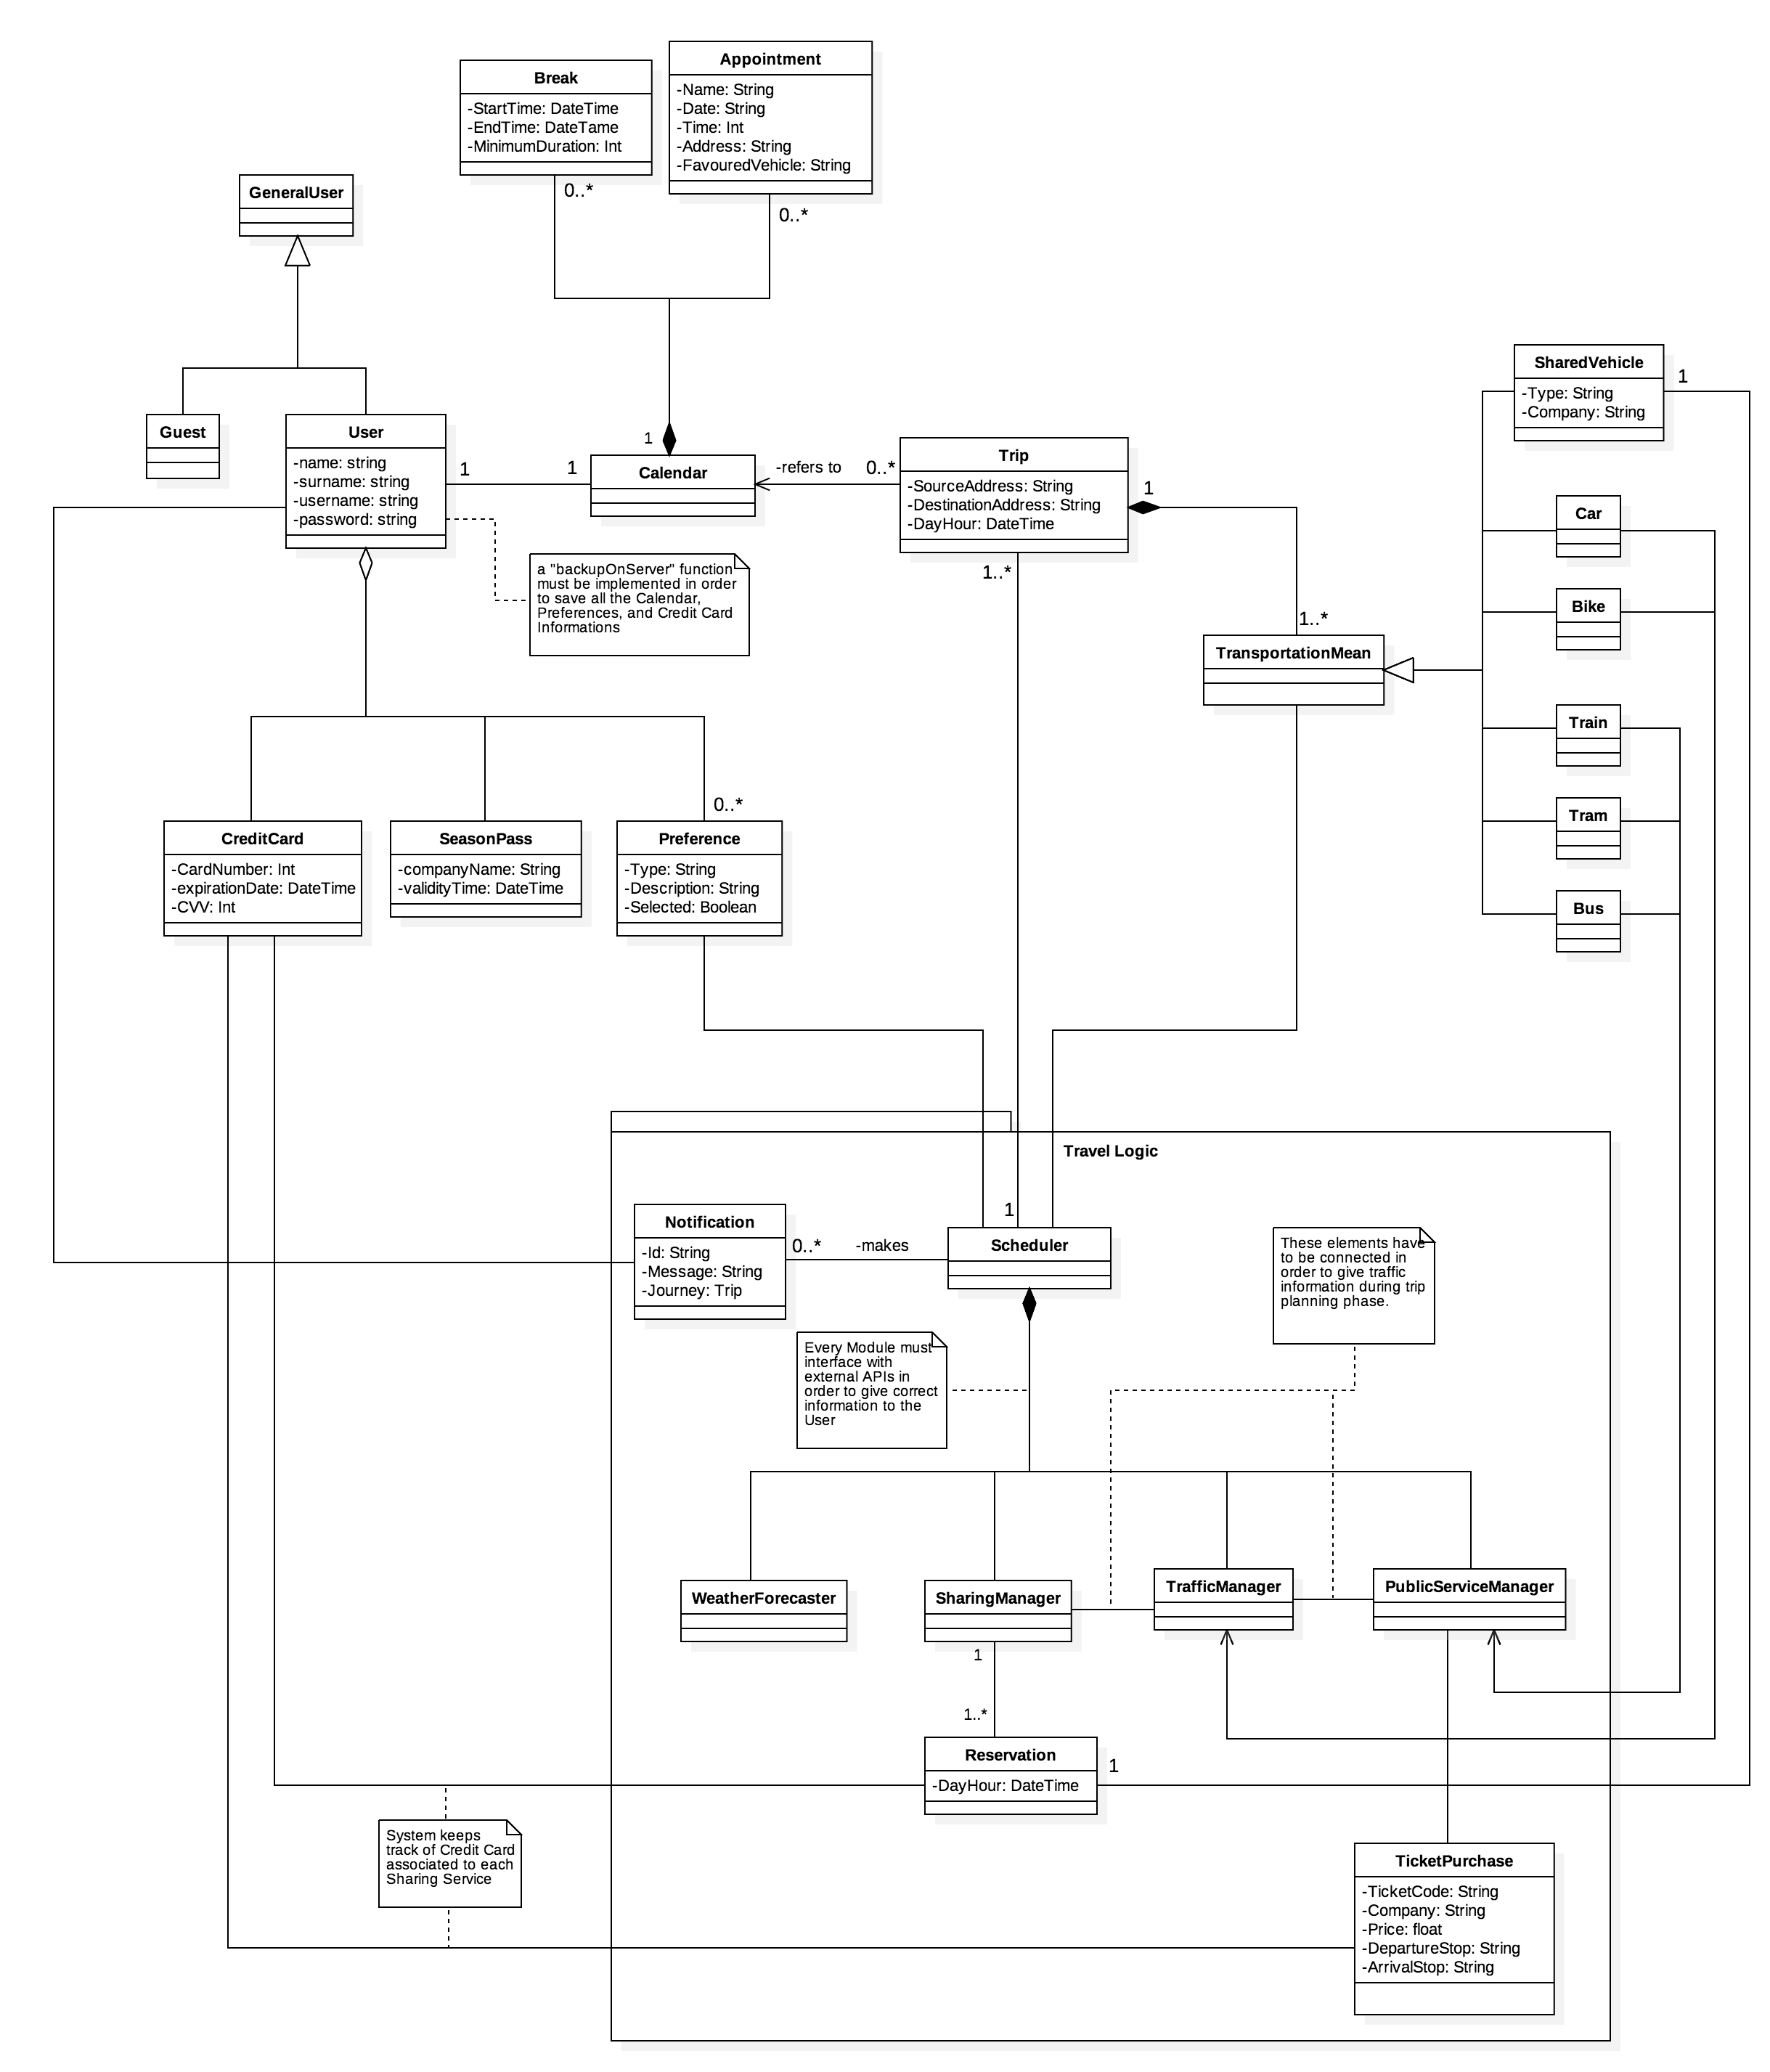
\includegraphics[width=\textwidth]{uml/classDiagram}
		\end{figure}				
			
\subsection{Product functions}
	
 We’ve already detailed the main goals of our mobile application in the first section of the current document; naturally, the aforementioned goals will be functions of \textit{Travlendar+}.
Here though we submit an higher-level description of major functions to ease the understanding of our program to all interested parties.
		
		\begin{description}
			\item[Appointments Manager] 
			Our mobile application will let any registered user to view, create, modify and delete events, denoted by their type, their date and location.

			\item[Travel Scheduling] 
			When a new appointment is inserted in the application timetable an immediate check is performed whether the location of the event can be reached in the allotted time on foot, by car, or by public transportation (referencing, in lack of additional information, to their default behaviour according to the date and time of the day).
			Day by day, events and allotted times are periodically checked with live informations to ensure they’re feasible : a list of results is prompted to the user whenever he asks for it and he can express preferences and filter them.
			
			\item[Payment Manager for Public Transportation]
			Our mobile application will redirect registered users to payment portals through secure channels and it’ll be able to verify whether transaction succeeded or not by interfacing with external payment services.
			Unfulfilled payment will result in an impossibility to go forward and will prompt the possibility to submit the data and restart the transaction.

			\item[Car and Bike Sharing Integration]
			The mobile app will be able to integrate external info about the availability and location of shared cars and bikes so that it will also allow their reservation.
			Everything past this mark clearly outgrows the scope of our system and it shall be handled by the company that grants the service (same goes for eventual malfunctions or erratic behaviours). 
			Travlendar+ will send send reservation requests to the selected company and will be able to record a rental acceptance notification (i.e., everything’s gone right in the provider’s rental system).


			\item[Free Time spans]
			Our system will grant the possibility to reserve free time spans :
			such breaks won’t be affected by scheduling and by the need to travel and registered users will be able to insert theme directly in the calendar.

	\end{description}

			
\subsection{User characteristics}
	We list the actors involved in our system :
	\begin{description}
		\item[Guest] A guest is a potential user, an unregistered or not-yet-logged person who opens the app. He can't access all its functionalities and, until it's logged in, his only choice is logging.
		\item[Registered User/User] The user is the final and only customer of \textit{Travlendar+;} he has identifying credentials, can personalize his timetable by setting up and configuring events, can specify favourite transportation means, buy tickets, view expected arrival times, reserve shared vehicles and get notified by the system.

	\end{description}
	In addition to that, \textit{Travlendar+} also interacts with different service providers :
	\begin{description}
		\item[Payment Service] Providers that cover transactions prompted by the mobile application
		\item[Localization Service] The provider that manages localization, maps and standard travel times 
		\item[Sharing Service] Service providers of car and bike sharing services that manage position and rental of vehicles
		\item[Public Transportation Service] Public Transportation information systems that show and sell tickets through \textit{Travlendar+}
	\end{description}

\subsection{Assumptions, dependencies and constraints}

We've already given a formal and methodical definition of our problem, yet there are still some ambiguities which still need to be addresed.


	\begin{enumerate}
		
			\item Users do not create events outside the “operative zone”

			\item The devices \textit{Travlendar+} is installed on possess a well-functioning GPS for geo-localization

			\item If a registered User is willing to use the vehicle of a sharing network, we assume him to have downloaded the corresponding sharing-network app

			\item There’s no kind of dependency among the users of our system

			\item Any information coming from sharing services regarding position, rental, and payment won’t be double-checked by our system

			\item Information coming from external payment sites won’t be double checked by our system

			\item Buying public transportation tickets rely on the aforementioned external payment procedures

			\item System assumes the season passes submitted by the user only aid for filtering results and are not checked nor have any legal value

			\item System assumes that any car rental request is made by a person who’s allowed to make one. Only sharing services check the validity of documents; in addition to that we always assume the driver is the user who requests the rental

			\item The application doesn't act as a navigator, and isn't capable of giving live informations about the travel besides the ones that can arrive through notifications
			
			\item Personal vehicles consider as their starting position the one of the geo-localized device
			
			\item Modified and deleted events cannot be restored in any way
			
			\item In order to use a vehicle sharing service its corresponding mobile application must be installed on the user device 
			
		\end{enumerate}
